\documentclass{article}

\setlength{\parskip}{1em}
\setlength{\parindent}{0pt}

% Formatting and images 
\usepackage[utf8]{inputenc}
\usepackage[margin=1in]{geometry}
\usepackage[titletoc,title]{appendix}
\usepackage{authblk}
\usepackage{graphicx}
\usepackage{hyperref}
\usepackage{url}

%% Language and font encodings
\usepackage[english]{babel}
\usepackage[T1]{fontenc}
\usepackage{booktabs}

%% Packages for mathematical typesetting
\usepackage{amsmath}
\usepackage{amsthm}
\usepackage{amssymb}
\usepackage{gensymb}
\usepackage{pgf}
\usepackage{comment}
\usepackage{float}
\usepackage{blindtext}
\usepackage{enumitem}
\usepackage{bbm}
\usepackage{array}
\newcommand*{\horzbar}{\rule[.5ex]{2.5ex}{0.5pt}}

\allowdisplaybreaks

\usepackage{algorithm2e}
\usepackage{algpseudocode}
\SetKwComment{Comment}{/* }{ */}
\RestyleAlgo{ruled}

\newtheorem{theorem}{Theorem}
\newtheorem{lemma}{Lemma}

% Title content
\title{MATH 480 Final Project}
\author[]{Max Ranis}
\author[]{Henry Smith}
\author[]{Andrew Wei}
\affil[]{\normalsize Yale University}

\date{\today}

\begin{document}

\maketitle

% Abstract
\begin{abstract}
    \noindent We prove that for any set of $n$ points $V$ in $\mathbb{R}^d$, there exists an embedding $f: \mathbb{R}^d \rightarrow \mathbb{R}^k$ for $k = \lceil 4(\epsilon^2/2 - \epsilon^3/3)^{-1} \log(n) \rceil$ that preserves the $\ell^2$ distance between any two points $x, y \in V$ within a factor of $\epsilon$ of their original distance. This result was first proven by Johnson and Lindenstrauss in 1984 and has numerous contemporary applications in machine learning.
\end{abstract}

% Introduction and Overview

\pagebreak

\section{The Johnson-Lindenstrauss Lemma}

\subsection{Historical Background}
In 1984, Johnson and Lindenstrauss published their seminal result regarding the random embedding of high-dimensional [Euclidean] data in lower-dimensional space. William Johnson is an American mathematician and has held positions at the University of Houston, Ohio State University, and Texas A\&M University, where he is currently the chair of the mathematics department. He was award the Stefan Banach Medal for his achievement in mathematics by the Polish Academy of Sciences in 2007. Joram Lindenstrauss was an Israeli mathematician who obtained his Ph.D. from the Hebrew University of Jerusalem in 1962. He thereafter worked as a postdoc at the Yale Mathematics department from 1962-1965. Two of his children went on to become mathematicians, and his son, Elon Lindenstrauss, was the first Israeli mathematician to win the Fields Medal in 2010. The Fields Medal was awarded for his work in ergodic theory and its applications to number theory. He now holds a professorship in the Princeton University Department of Mathematics.

\subsection{Preliminaries}
Let $\left\Vert \cdot \right\Vert$ denote the $\ell^2$ (Euclidean norm); we consider the Banach spaces $(\mathbb{R}^d, \left\Vert \cdot \right\Vert), (\mathbb{R}^k, \left\Vert \cdot \right\Vert)$ where $d > k$. Further, let $\mathcal{N}(0, 1)$ denote the standard normal distribution in $\mathbb{R}$ with density $f(x) = \frac{1}{\sqrt{2 \pi}} \exp \left(-\frac{x^2}{2} \right)$. Likewise let, $\mathcal{N}(\boldsymbol{0}, \mathbb{I}_p)$ denote the standard multivariate normal distribution in $\mathbb{R}^p$ with density $f_p(x) = \prod_{i=1}^p f(x) = \frac{1}{(2 \pi)^{p/2}} \exp \left(-\frac{1}{2} \left\Vert x \right\Vert^2 \right)$.

\subsection{Problem Statement}

\begin{theorem} \textbf{(Johnson-Lindenstrauss)}\\
    For any $0 < \epsilon < 1$ and any integer $n$, let $k$ be a positive integer such that
    \begin{align*}
        k \geq 4(\epsilon^2/2 - \epsilon^3/3)^{-1} \log(n).
    \end{align*}
    Then for any set $V$ of $n$ points in $\mathbb{R}^d$, there is a map $f: \mathbb{R}^d \rightarrow \mathbb{R}^k$ such that for all $x_i, x_j \in V$,
    \begin{align*}
        (1 - \epsilon) \left \Vert x_i - x_j \right \Vert^2 \leq \left \Vert f(x_i) - f(x_j) \right \Vert^2 \leq (1 + \epsilon) \left \Vert x_i - x_j \right \Vert^2.
    \end{align*}
    Furthermore, this map can be found in randomized polynomial time \cite{dasgupta1999elementary}.
\end{theorem}

\noindent
Here, $k$ is the dimension of the space onto which which we are projecting our $n$ points in $\mathbb{R}^d$. The second inequality tells us that the mapping $f: \mathbb{R}^d \rightarrow \mathbb{R}^k$ will preserve the distance between any two points within a factor of $\epsilon$ of their original distance in $\mathbb{R}^d$. If we would like a greater preservation of the $\ell^2$ distances between points, then we would need to decrease $\epsilon$. This, in turn, would increase the dimension $k$ of the space onto which we are projecting.

\section{Proof}

\subsection{Random Projections onto $\mathbb{R}^k$}\label{ss1:randproj}

The map $f$ we wish to find takes points $v \in V \subset \mathbb{R}^d$ to $f(v) \in \mathbb{R}^k$. Accordingly, we would like to identify a $k$-dimensional subspace of $\mathbb{R}^d$ onto which we can map our set of points. Since the result must hold for \textit{any} subset $V$ of $n$ points in $\mathbb{R}^d$, then constructing a $k$-dimensional subspace deterministically would be a futile effort. Rather, we project each $v \in V$ onto a \textit{random} $k$-dimensional subspace of $\mathbb{R}^d$ as follows:

Consider the vectors $A_i \in \mathbb{R}^d$, $1 \le i \le k$, defined to have entries $(A_i)_j \overset{i.i.d.}{\sim} \mathcal{N}(0, 1)$ for $1 \le j \le d$. In other words, we need $k\times d$ independent random values, each drawn from the standard normal distribution. See Appendix \ref{stdnorm} for an in-depth discussion of how one could generate normally-distributed values using the $\text{Uniform}(0,1)$ distribution. Note that with probability $1$, $\text{span}\left(A_1, \ldots, A_k \right)$ is a $k$-dimensional subspace of $\mathbb{R}^n$. Now, assuming that we have these $k$ random vectors, we will consider a projection matrix $\mathbb{A} \in \mathbb{R}^{k \times d}$ where each row is one of the $k$ vectors:
\begin{align*}
        \mathbb{A} = 
        \left[
            \begin{array}{ccc}
            \horzbar & A_{1} & \horzbar \\
            \horzbar & A_{2} & \horzbar \\
            & \vdots &  \\
            \horzbar & A_{k} & \horzbar
            \end{array}
        \right]
\end{align*}

With this random matrix $\mathbb{A} \in \mathbb{R}^{k \times n}$, we construct the map $f: \mathbb{R}^d \rightarrow \mathbb{R}^k$ defined $f(x) := \frac{1}{\sqrt{k}}\mathbb{A}x$ for $x \in \mathbb{R}^d$.

    \begin{figure}[H]
        \centering
        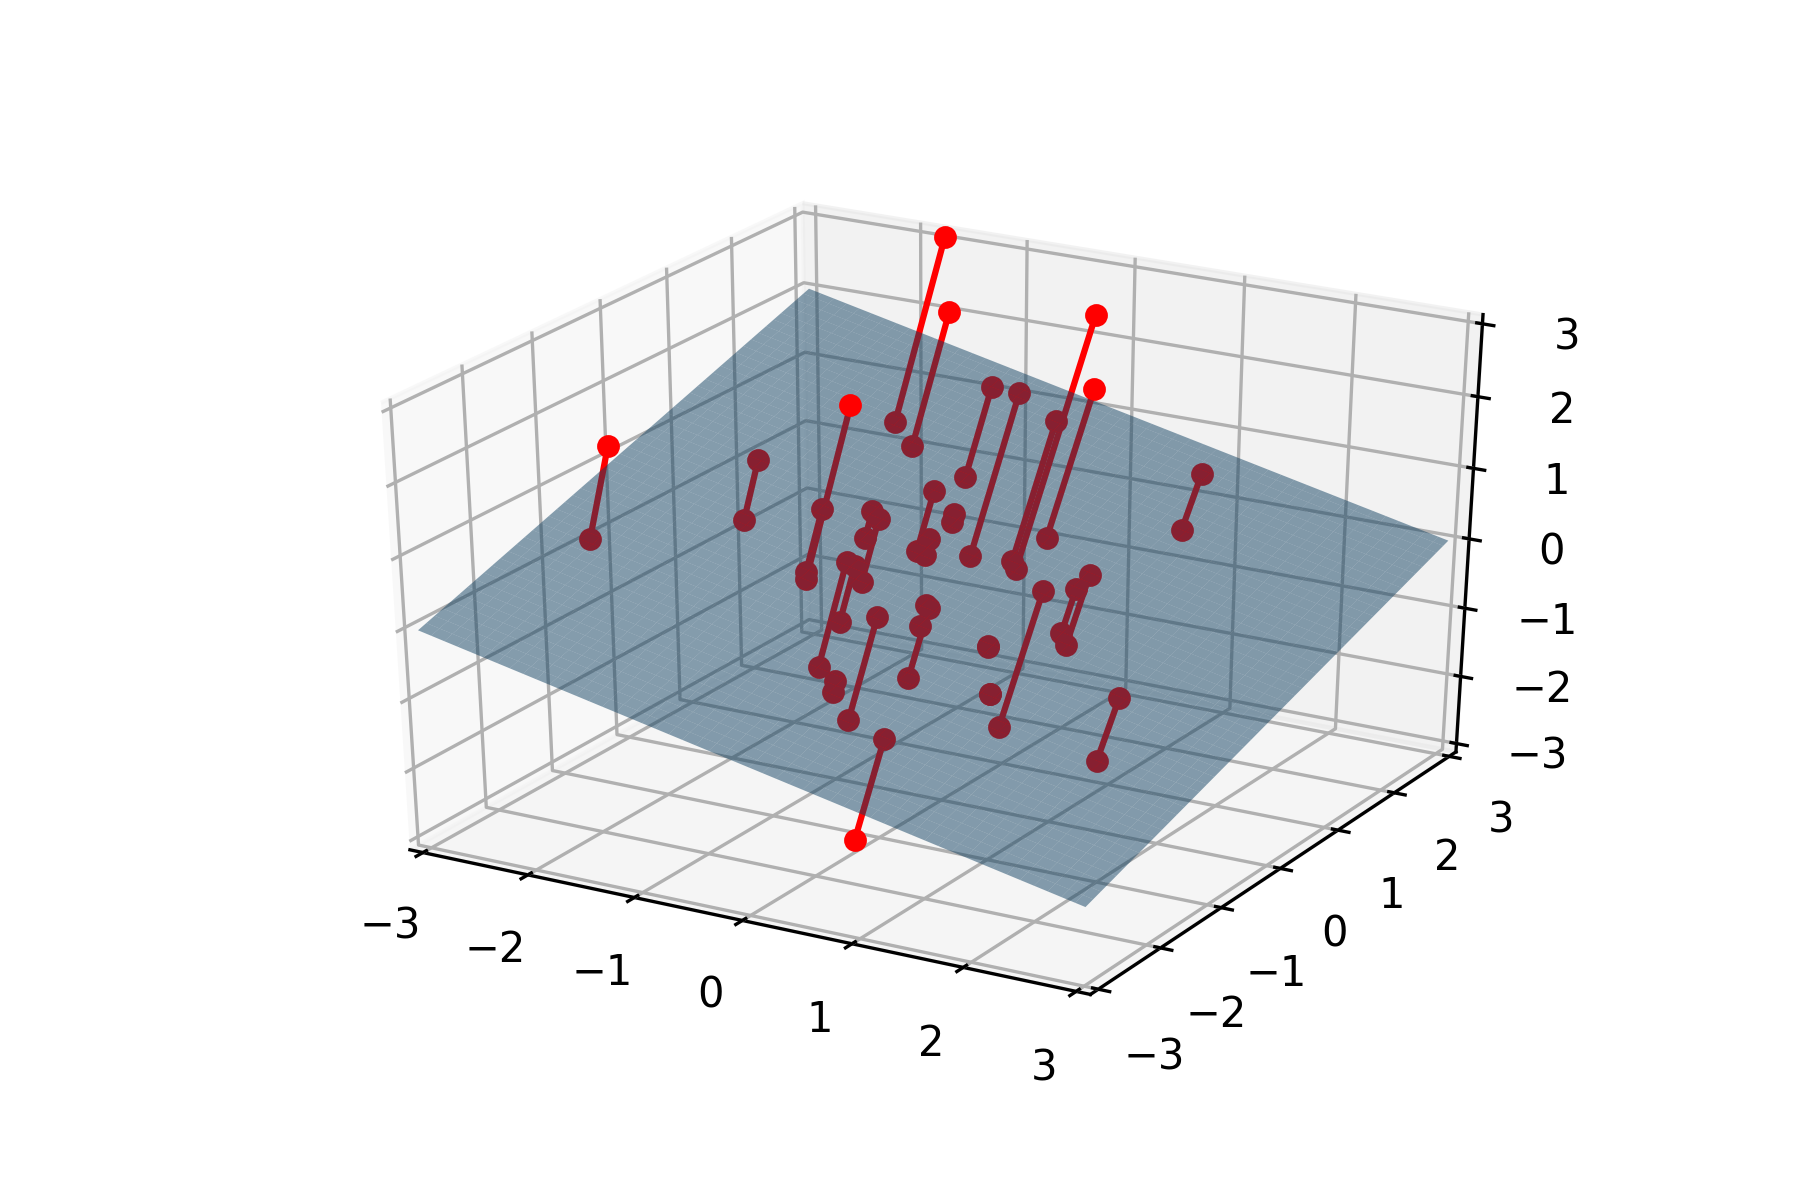
\includegraphics[width=\textwidth]{imgs/random_projections.png}
        \caption{The projection of $n = 50$ random points in $\mathbb{R}^3$ onto a two-dimensional hyperplane determined by the random Gaussian vectors $A_1, A_2 \in \mathbb{R}^3$. Note that $\frac{1}{\sqrt{k}} \mathbb{A} \in \mathbb{R}^{k \times d}$ is the \textit{orthogonal projection matrix} corresponding to some $k$-dimensional subspace $\mathcal{S}$ of $\mathbb{R}^d$; that is, $f(u) = \frac{1}{\sqrt{k}}\mathbb{A}u$ maps each vector $u \in \mathbb{R}^d$ to its orthogonal projection onto $\mathcal{S}$.}
    \end{figure}
    
    \subsection{The Distribution of $f(u) \in \mathbb{R}^k$}

    Let $y := f(u)$, where $f: \mathbb{R}^d \rightarrow \mathbb{R}^k$ is defined as in section (\ref{ss1:randproj}). Since $\mathbb{A}$ is a matrix with random entries and $y$ is a linear transformation of $\mathbb{A}$, then it must also be true that $y \in \mathbb{R}^k$ is a random vector. Thus, we can consider the distribution of $y \in \mathbb{R}^k$, which is the subject of the following lemma:
    
    \begin{lemma}\label{lm:1}
    Let $y := f(u) \in \mathbb{R}^k$. Then $y \sim \frac{\left \Vert u \right \Vert}{\sqrt{k}} Z$, where random vector $Z$ has density $\mathcal{N}(\boldsymbol{0}, \mathbb{I}_k).$
    \end{lemma}
    \begin{proof}
    First, we note that $y_i = \frac{1}{\sqrt{k}} \mathbb{A}_{i,:}u = \sum_{j=1}^d \frac{1}{\sqrt{k}} \mathbb{A}_{i,j} u_j = \sum_{j=1}^d \left(\frac{u_j}{\sqrt{k}} \right) A_{i,j}$. Since $A_{i,1}, \ldots, A_{i,d} \overset{i.i.d.}{\sim} \mathcal{N}(0, 1)$ and each $\left(\frac{u_j}{\sqrt{k}} \right) \in \mathbb{R}$ is non-random, then $y_i$ is normally distributed. That is, $y_i$ is normally distributed since it is the sum of independent normally-distributed random variables. Further, because each $y_i$ is a function of $A_{i,1}, \ldots, A_{i,d}$ and $A_{i, j} \overset{i.i.d.}{\sim} \mathcal{N}(0, 1)$ for $1 \le i \le k$, $1 \le j \le d$ (i.e. both the rows and the columns of $\mathbb{A}$ are i.i.d. normal random variables), then we also have that $y_1, \ldots, y_k$ are independent and identically distributed. 
    
    \noindent
    It is not in general true that each $y_i$ normally distributed implies that $y = (y_1, \ldots, y_k)$ has a multivariate normal distribution. Since each $y_1, \ldots, y_k$ is independent, however, this is, in fact, true. This is because each linear combination $a_1y_1 + \ldots + a_ky_k$ is normally distributed and so, by definition, $y$ has multivariate normal density. It remains to find the expectation and covariance matrix of multivariate normal random variable $y$. For the expectation, we have
    \begin{align*}
        \mathbb{E}(y_i) &= \mathbb{E} \left( \sum_{j=1}^d \left(\frac{u_j}{\sqrt{k}} \right) A_{i,j} \right)\\
                        &= \sum_{j=1}^d \mathbb{E}\left( \frac{u_j}{\sqrt{k}}A_{i,j}  \right) &\text{linearity of expectation}\\
                        &= \sum_{j=1}^d \frac{u_j}{\sqrt{k}} \mathbb{E}\left(A_{i,j} \right) &\text{linearity of expectation}\\
                        &= 0. &A_{i,j} \sim \mathcal{N}(0, 1)
    \end{align*}
    
    Now for the covariance matrix of $y \in \mathbb{R}^k$, note that $y_i, y_j$ independent for $i \neq j$ implies $y_i, y_j$ uncorrelated. And since the $y_i$'s are identically distributed, then the covariance of $y$ is of the form $a\mathbb{I}_k$ for $a = \text{var}(y_i)$.
    \begin{align*}
        \text{var}(y_i) &= \text{var} \left( \sum_{j=1}^d \left(\frac{u_j}{\sqrt{k}} \right) A_{i,j} \right)\\
                        &= \sum_{j=1}^d \text{var} \left(\frac{u_j}{\sqrt{k}}A_{i,j} \right) &\text{$A_{i,1}, \ldots, A_{i,d}$ independent}\\
                        &= \sum_{j=1}^d \frac{u_j^2}{k} \text{var} \left(A_{i,j} \right) &\text{properties of variance}\\
                        &= \sum_{j=1}^d \frac{u_j^2}{k} &A_{i,j} \sim \mathcal{N}(0,1)\\
                        &= \frac{1}{k} \sum_{j=1}^d u_j^2\\
                        &= \frac{\left \Vert u \right \Vert^2}{k}.
    \end{align*}
    \end{proof}
    
     Furthermore, we can say something about the distribution of $\left\Vert y \right\Vert^2$:
     \begin{lemma}
     $\mathbb{E} \left\Vert y \right\Vert^2 = \left\Vert u \right\Vert^2$ where $y:= f(u)$.
     \end{lemma}
     
     \begin{proof}
     \begin{align*}
         \mathbb{E}(\left\Vert y \right\Vert^2) &= \mathbb{E} \left(\sum_{i=1}^k y_i^2\right)\\
         &= \mathbb{E} \left(\sum_{i=1}^k \left( \sum_{j=1}^d \frac{u_j}{\sqrt{k}}A_{i,j} \right)^2\right) &\text{def. of $y = f(u)$}\\
         &= \frac{1}{k} \mathbb{E} \left(\sum_{i=1}^k \left( \sum_{j=1}^d u_j A_{i,j} \right)^2\right) &\text{linearity of expectation}\\
         &= \frac{1}{k} \sum_{i=1}^k \mathbb{E} (u_1A_{i,1} + \ldots + u_dA_{i,d}) \cdot (u_1A_{i,1} + \ldots + u_dA_{i,d}).
     \end{align*}
     
     Now, since $A_{i,k_1}, A_{i,k_2}$ are independent for $k_1 \neq k_2$, then $\mathbb{E}(u_{k_1}u_{k_2}A_{i,k_1}A_{i,k_2}) = u_{k_1}u_{k_2} \mathbb{E}(A_{i,k_1}A_{i,k_2}) = u_{k_1}u_{k_2} \mathbb{E}(A_{i,k_1})\mathbb{E}(A_{i,k_2}) = 0$ whenever $k_1 \neq k_2$. This allows us to simplify our expression for $\mathbb{E}(\left\Vert y \right\Vert^2)$:
     \begin{align*}
         &\frac{1}{k} \sum_{i=1}^k \mathbb{E} (u_1A_{i,1} + \ldots + u_dA_{i,d}) \cdot (u_1A_{i,1} + \ldots + u_dA_{i,d})\\
         &= \frac{1}{k} \sum_{i=1}^k \sum_{j=1}^d \mathbb{E}(u_j^2 A_{j,j}^2)\\
         &= \frac{1}{k} \sum_{i=1}^k \sum_{j=1}^d u_j^2 \mathbb{E}(A_{j,j}^2) &\text{linearity of expectation}\\
         &= \frac{1}{k} \sum_{i=1}^k \sum_{j=1}^d u_j^2 \text{Var}(A_{j,j}) & \mathbb{E}(A_{j,j}) = 0\\
         &= \frac{1}{k} \sum_{i=1}^k \sum_{j=1}^d u_j^2 &A_{j,j} \sim \mathcal{N}(0,1)\\
         &= \frac{1}{k} \cdot k \sum_{j=1}^d u_j^2\\
         &= \left\Vert u \right\Vert^2.
     \end{align*}
     \end{proof}

    From our understanding of the multivariate normal density, the projection of vector $u$ onto the  $k$-dimensional subspace determined by $\mathbb{A}$ has, with high probability, squared $\ell^2$ norm clustered around that of $u$.
    \begin{figure}[H]
        \centering
        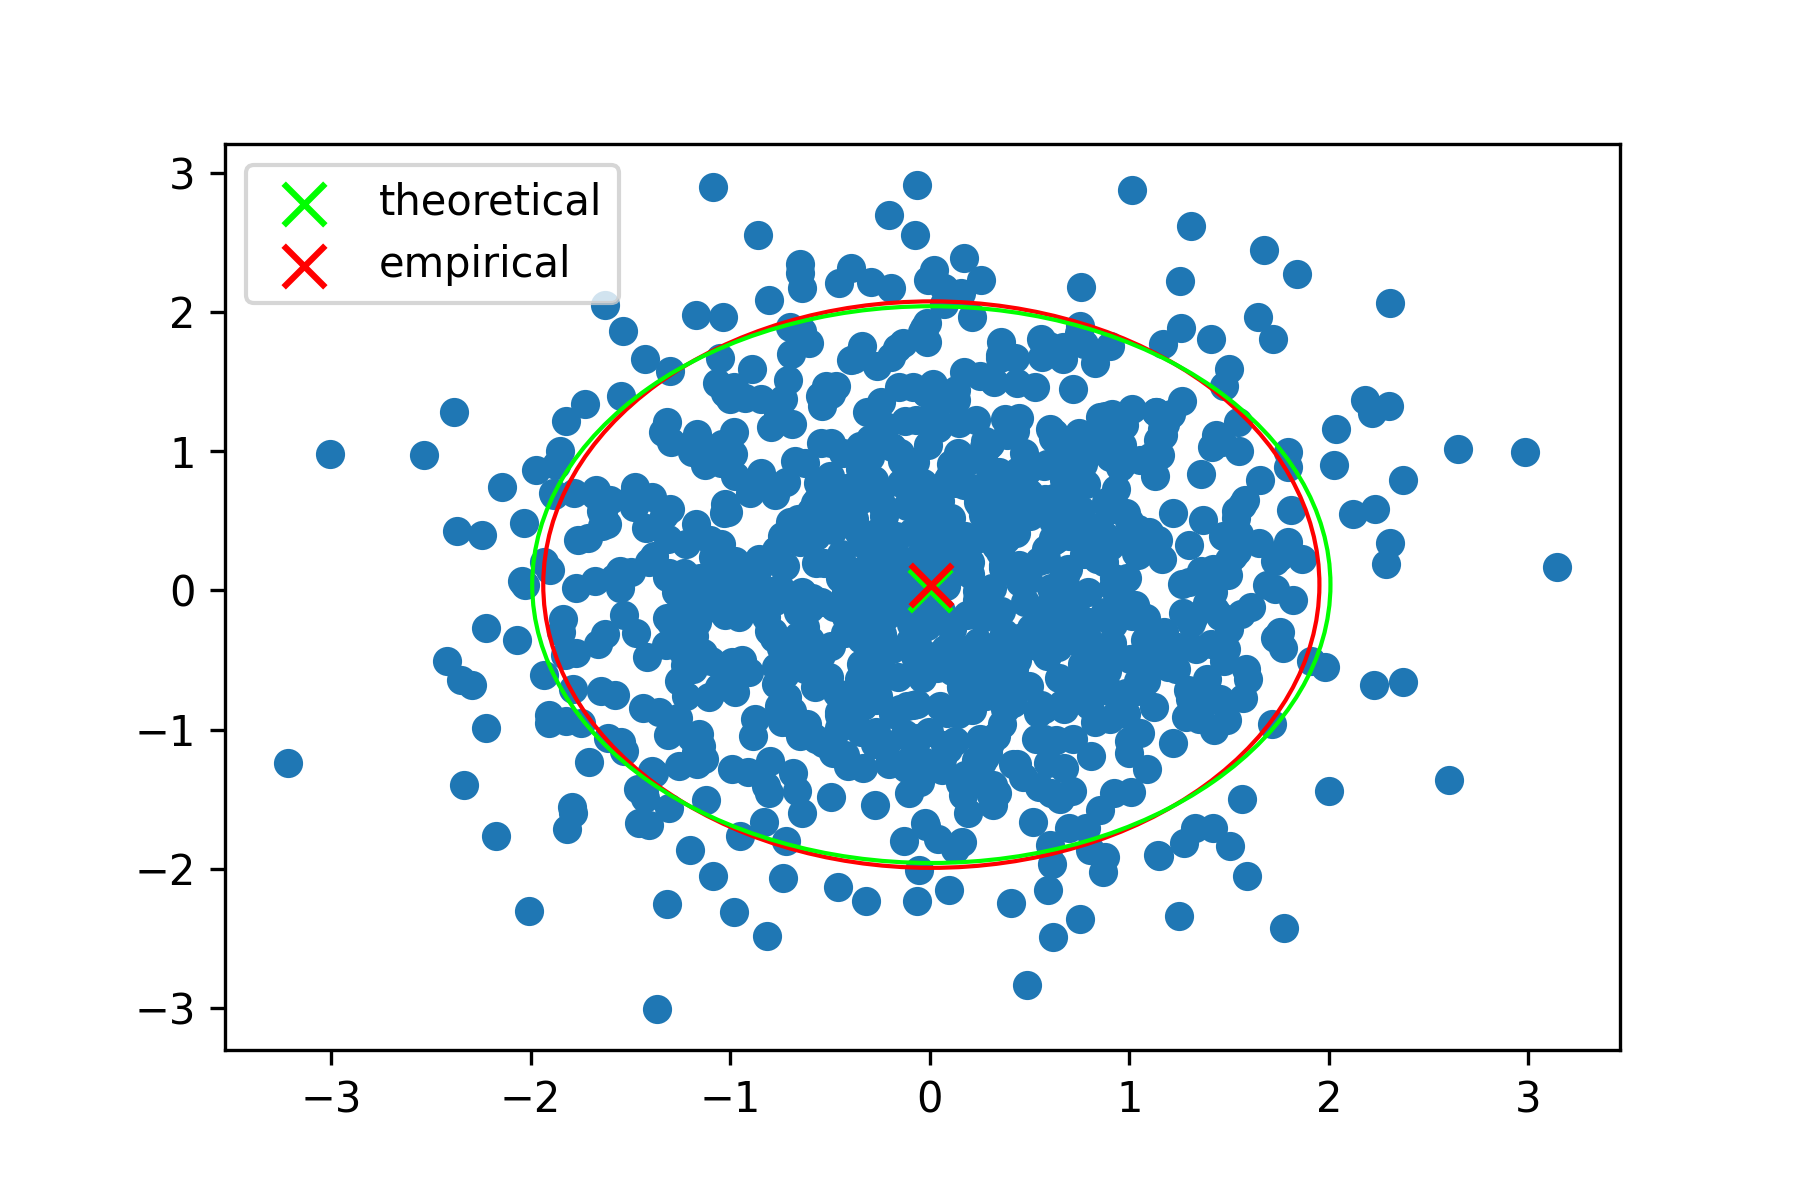
\includegraphics[width=\textwidth]{imgs/projectpts2d.png}
        \caption{$N = 10^4$ simulated projections of the vector $u = \mathbbm{1} \in \mathbb{R}^5$ onto a two-dimensional subspace according to $f(u) = \frac{1}{\sqrt{k}}\mathbb{A}u$, where $\mathbb{A}$ is randomly generated as described in (\ref{ss1:randproj}) upon each iteration. In green is the theoretical distribution of $\frac{\sqrt{k}}{\left \Vert u \right \Vert}f(u) \sim \mathcal{N}(\boldsymbol{0}, \mathbb{I}_k)$ derived in Lemma \ref{lm:1} and in red is the empirical distribution. Ellipses represent the regions in which approximately $95$\% of the projections lie.}
    \end{figure}
    
\subsection{Calculating Tail Probabilities}

To substantiate our prior observation about the distribution of $\left \Vert y \right \Vert^2$, we show the following result:

\begin{theorem}\label{thm:2}
    Let $y:= f(u)$, where $f: \mathbb{R}^d \rightarrow \mathbb{R}^d$ is defined as above. Then we have that 
    \begin{align*}
        \mathbb{P}\bigg[ \left\Vert y \right\Vert^2 \notin \left[(1 - \epsilon)\left\Vert u \right\Vert^2, (1 + \epsilon)\left\Vert u \right\Vert^2 \right] \bigg] \leq \frac{2}{n^2}.
    \end{align*}
\end{theorem}

This means the probability that $\left\Vert y \right\Vert^2$ is more than a factor of $\epsilon$ from $\left\Vert u \right\Vert^2$ is less than or equal to $\frac{2}{n^2}$.

\begin{proof}

To begin, we standardize the vector $y \in \mathbb{R}^k$. Particularly, let us define
$$ \hat{u} = \frac{u}{\left\Vert u \right\Vert}, \quad v = \frac{1}{\left\Vert u \right\Vert}\mathbb{A}u = \mathbb{A} \hat{u}.$$

Then from Lemma \ref{lm:1} we have that

$$ v_i =  \mathbb{A}_{i,:}^T \frac{u}{\left\Vert u \right\Vert} \overset{i.i.d.}{\sim} \mathcal{N}(0, 1).$$

To express this standard multivariate normal vector $v$ in terms of $y$, notice that $y = \mathbb{A}u/\sqrt{k} \Rightarrow \mathbb{A}u = \sqrt{k}y$. This means that
$$ v = \frac{\sqrt{k}y}{\left\Vert u \right\Vert^2} \Rightarrow \left\Vert v \right\Vert^2 = k \frac{\left\Vert y \right\Vert^2}{\left\Vert u \right\Vert^2}.$$

\subsubsection{Finding the upper bound for  $\mathbb{P} \left[ \left\Vert y \right\Vert^2_2 \geq (1+\epsilon) \left\Vert u \right\Vert^2_2 \right]$}
For short-hand, let $\lambda = \frac{\epsilon}{2(1+\epsilon)} > 0.$ Then we have that
\begin{align*}
\mathbb{P}[\left\Vert y \right\Vert^2 \geq (1+\epsilon) \left\Vert u \right\Vert^2] & = \mathbb{P} \left[\frac{\left\Vert u \right\Vert^2 \left\Vert v \right\Vert^2}{k} \geq (1+\epsilon) \left\Vert u \right\Vert^2 \right] & \text{above expression for $\left\Vert v \right\Vert^2 $}\\
& = \mathbb{P} \left[ \left\Vert v \right\Vert^2 \geq (1+\epsilon) k \right] \\
& = \mathbb{P}\left[ \exp(\lambda \left\Vert v \right\Vert^2) \geq \exp(\lambda (1+\epsilon) k) \right]. & \text{since $\lambda > 0$}
\end{align*}
By Markov's Inequality, we know that $\mathbb{P}[Y \geq a] \leq \mathbb{E}[Y]/a$ for any random variable $Y$:
\begin{align*}
\mathbb{P} \left[ \left\Vert y \right\Vert^2 \geq (1+\epsilon) \left\Vert u \right\Vert^2 \right] \leq \frac{\mathbb{E}\left[\exp(\lambda \left\Vert v \right\Vert^2) \right] }{ \exp(\lambda (1+\epsilon) k)} = \frac{\mathbb{E}\left[\exp(\lambda \sum_{i=1}^k v_i^2) \right]}{ \exp(\lambda (1+\epsilon) k)} = \frac{\mathbb{E}\left[\prod_{i=1}^k \exp(\lambda  v_i^2) \right]}{ \exp(\lambda (1+\epsilon) k)}.
\end{align*}
Since we know that the $v_i$'s are independent and identically-distributed, then
\begin{align*}
\mathbb{P} \left[ \left\Vert y \right\Vert^2 \geq (1+\epsilon) \left\Vert u \right\Vert^2 \right] \leq \frac{\prod^k_{i=1} \mathbb{E} \left[ \exp(\lambda v_i^2) \right]}{\exp(\lambda (1+\epsilon) k)} = \bigg (\frac{ \mathbb{E} \left[\exp(\lambda v_i^2) \right] }{ \exp(\lambda (1+\epsilon))} \bigg)^k.
\end{align*}
Now, because $v_i \sim \mathcal{N}(0, 1)$, then $v_i^2 \sim \chi_1^2$. That is, $v_i^2$ is distributed as chi-square with one degree of freedom. As we show in the appendix, for $X \sim \chi_1^2$, then $\mathbb{E}\exp(tx) = (1-2t)^{-1/2}$ for $t < 1/2$. Here, $\mathbb{E}\exp(tx)$ is called the \textit{moment-generating function} (MGF) of $X$. Since $0< \lambda < 1/2$ for $0 < \epsilon < 1$, then we have
\begin{align*}
\mathbb{P}\left[ \left\Vert y \right\Vert^2 \geq (1+\epsilon) \left\Vert u \right\Vert^2 \right] \leq \bigg(  \frac{ 1 }{ \exp(\lambda (1+\epsilon)) \sqrt{1-2\lambda} } \bigg)^k.
\end{align*}
Then, substituting in $\lambda = \frac{\epsilon}{2(1+\epsilon)}$,
\begin{align*}
\mathbb{P}\left[ \left\Vert y \right\Vert^2 \geq (1+\epsilon) \left\Vert u \right\Vert^2 \right] \leq \bigg(   \exp(-\epsilon) (1+\epsilon)  \bigg)^{k/2} = \bigg(  \exp(-\epsilon + \log(1+\epsilon) )  \bigg)^{k/2}.
\end{align*}
As we discuss in the appendix, for $x \in (0,1)$, $\log(1+x)$ is bounded above by odd orders of its Taylor expansion. This allows us to write $\log(1+ \epsilon) \leq \epsilon - \epsilon^2/2 + \epsilon^3/3$ for $0 < \epsilon < 1$, which means that
\begin{align*}
\mathbb{P} \left[ \left\Vert y \right\Vert^2 \geq (1+\epsilon) \left\Vert u \right\Vert^2 \right] \leq \bigg( \exp(-\epsilon + \epsilon - \epsilon^2/2 + \epsilon^3/3 )  \bigg)^{k/2} = \exp( - \epsilon^2/2 + \epsilon^3/3 )^{k/2}.
\end{align*}
Recall that, by assumption, we have $k \geq 4(\epsilon^2/2 - \epsilon^3/3)^{-1} \log(n)$. This means that $(k/4)\log(n) \geq (\epsilon^2/2 - \epsilon^3/3)^{-1}$, or alternatively $4\log(n)/k \geq (\epsilon^2/2 - \epsilon^3/3)$. We thus conclude
\begin{align*}
\mathbb{P}\left[ \left\Vert y \right\Vert^2 \geq (1+\epsilon) \left\Vert u \right\Vert^2 \right] \leq \exp( - \epsilon^2/2 + \epsilon^3/3 )^{k/2} \leq \exp( - 4 \log(n) / k )^{k/2} = \exp(-2 \log(n)) = n^{-2}.
\end{align*}
        
\subsubsection{Finding the upper bound of $\mathbb{P} \left[ \left\Vert y \right\Vert^2 \leq (1-\epsilon) \left\Vert u \right\Vert^2 \right]$}

We use a similar method to prove the desired upper bound. This time, let $\lambda = \frac{\epsilon}{2(1-\epsilon)}.$  Then we have 
\begin{align*}
\mathbb{P} \left[ \left\Vert y \right\Vert^2 \leq (1-\epsilon) \left\Vert u \right\Vert^2 \right] & = \mathbb{P} \left[ \frac{\left\Vert u \right\Vert^2 \left\Vert v \right\Vert^2}{k} \leq (1-\epsilon) \left\Vert u \right\Vert^2 \right]\\
& = \mathbb{P} \left[\exp(\lambda \left\Vert v \right\Vert^2) \leq \exp(\lambda (1-\epsilon) k) \right] & \text{since $\lambda > 0$}\\
& = \mathbb{P} \left[ \exp( - \lambda \left\Vert v \right\Vert^2) \geq \exp( - \lambda (1-\epsilon) k) \right] \\
& \leq \frac{\mathbb{E}[\exp( - \lambda \left\Vert v \right\Vert^2)]}{\exp( - \lambda (1-\epsilon) k)}  & \text{Markov's inequality}\\
 & = \frac{\mathbb{E}[\exp( - \lambda \sum_{i=1}^k v_i^2)]}{\exp( - \lambda (1-\epsilon) )}\\
 &= \frac{\mathbb{E}[\exp( - \lambda \sum_{i=1}^k v_i^2)]}{\exp( - \lambda (1-\epsilon) )}\\
 &= \frac{\mathbb{E} \left[\prod_{i=1}^k \exp( - \lambda v_i^2) \right]}{\exp( - \lambda (1-\epsilon) )}\\
 &= \bigg( \frac{\mathbb{E}\exp(-\lambda v_i^2)}{\exp( - \lambda (1-\epsilon) )} \bigg)^k. & \text{$v_i$'s are i.i.d.}
\end{align*}
Since $v_i \sim \mathcal{N}(0, 1) \Rightarrow v_i^2 \sim \chi_1^2$, then we can once again use the moment-generating function (MGF) of $X \sim \chi_1^2$. The existence of the MGF relies on the fact that that $-\lambda < 1/2$ for $0 < \epsilon < 1$. Thus, we have
\begin{align*}
    \mathbb{P}\left[ \left\Vert y \right\Vert^2 \leq (1-\epsilon) \left\Vert u \right\Vert^2 \right] \leq \bigg(\frac{1}{ \exp(-\lambda (1-\epsilon)) \sqrt{1+2\lambda} } \bigg)^k.
\end{align*}
Substituting in $\lambda = \frac{\epsilon}{2(1-\epsilon)}$, we get
\begin{align*}
     \mathbb{P}\left[ \left\Vert y \right\Vert^2 \leq (1-\epsilon) \left\Vert u \right\Vert^2 \right] \leq \bigg( \frac{1}{\exp(-\epsilon)(1 - \epsilon)^{-1}} \bigg)^{k/2} = \bigg( \exp(\epsilon)(1 - \epsilon) \bigg)^{k/2} = \bigg( \exp(\epsilon + \log(1 - \epsilon)) \bigg)^{k/2}.
\end{align*}
Recall that $\log(1 - x)$ has the Taylor series expansion $- \sum_{n=1}^{\infty} \frac{x^n}{n}$ for $x \in [-1, 1)$. Since each term in the infinite sum is negative, then we can bound $\log(1 - x) = - \sum_{n=1}^{\infty} \frac{x^n}{n} \leq - x -x^2/2 \leq - x -x^2/2 + x^3/3$ for $x \in (0, 1)$. And so because $\epsilon \in (0,1)$, then we get that 
\begin{align*}
\mathbb{P}\left[ \left\Vert y \right\Vert^2 \leq (1-\epsilon) \left\Vert u \right\Vert^2 \right] &\leq \bigg(\exp(\epsilon - \epsilon - \epsilon^2/2 + \epsilon^3/3) \bigg)^{k/2}\\
& = \exp(-\epsilon^2/2 + \epsilon^3/3)^{k/2}.
\end{align*}
Finally, by our assumption that $k \geq 4(\epsilon^2/2 - \epsilon^3/3)^{-1} \log(n) \Rightarrow \epsilon^2/2 - \epsilon^3/3 \geq 4\log(n)/k \Rightarrow  -\epsilon^2/2 + \epsilon^3/3 \leq -4\log(n)/k$, then we conclude
\begin{align*}
    \mathbb{P}\left[ \left\Vert y \right\Vert^2 \leq (1-\epsilon) \left\Vert u \right\Vert^2 \right] \leq \exp(-4 \log(n)/k)^{k/2} = \exp(-2\log(n)) = n^{-2}.
\end{align*}

\subsubsection{Conclusion}
With these two upper bounds, we have
\begin{align*}
&\mathbb{P} \left[ \left\Vert y \right\Vert^2 \notin \left[(1 - \epsilon)\left\Vert u \right\Vert^2, (1 + \epsilon)\left\Vert u \right\Vert^2 \right] \right]\\
&= \mathbb{P} \left[ \left\Vert y \right\Vert^2 < (1 - \epsilon) \left\Vert u \right\Vert^2 \cup \left\Vert y \right\Vert^2 > (1 + \epsilon) \left\Vert u \right\Vert^2 \right] \\
&\leq \mathbb{P} \left[ \left \Vert y \right \Vert^2 < (1 - \epsilon) \left \Vert u \right \Vert^2\right] + \mathbb{P} \left[ \left \Vert y \right \Vert^2 > (1 + \epsilon) \left \Vert u \right \Vert^2\right]\\
&\leq \mathbb{P} \left[ \left \Vert y \right \Vert^2 \leq (1 - \epsilon) \left \Vert u \right \Vert^2\right] + \mathbb{P} \left[ \left \Vert y \right \Vert^2 \geq (1 + \epsilon) \left \Vert u \right \Vert^2\right]\\
&= \frac{2}{n^2}.
\end{align*}
\end{proof}

\subsection{A Union Bound}
Having proven the bulk of the lemma, we now consider our particular data $V = \{x_i\}_{i=1}^n \subseteq \mathbb{R}^d$. Let us take $u = x_i - x_j$ for $x_i, x_j \in V$ as well as  $y = f(u) = \frac{1}{\sqrt{k}} \mathbb{A}(x_i - x_j) = \frac{1}{\sqrt{k}} \mathbb{A}x_i - \frac{1}{\sqrt{k}} \mathbb{A}x_j = f(x_i) - f(x_j)$. Notice that we rewrote $f(u)$ using the linearity of $f: \mathbb{R}^d \rightarrow \mathbb{R}^k$. Then from Theorem \ref{thm:2} we know
    \begin{align*}
        \mathbb{P}\bigg[ \left\Vert f(x_i) - f(x_j) \right\Vert^2 \notin \left[(1 - \epsilon)\left\Vert x_i - x_j \right\Vert^2, (1 + \epsilon)\left\Vert x_i - x_j \right\Vert^2 \right] \bigg] \leq \frac{2}{n^2}.
    \end{align*}
    
Define $E_{i, j}$ to be the event that $x_i$ and $x_j$ satisfy the condition above. This event is the \textit{complement} of the desired distance distortion property for points $x_i$ and $x_j$. And so the event whose probability we would like to calculate is $\bigcap_{ \{i, j\} \in \binom{[n]}{2}} (E_{i, j})^c$ (\textit{all} pairs of points satisfy the distance distortion property). We use the complement rule as well as De Morgan's laws to express
\begin{align*}
    \mathbb{P} \left[\bigcap_{ \{i, j\} \in \binom{[n]}{2}} (E_{i, j})^c \right] = 1 - \mathbb{P} \left[\bigcup_{ \{i, j\} \in \binom{[n]}{2}} E_{i, j} \right].
\end{align*}
The probability of the event on the right-hand side of the equality satisfies
\begin{align*}
    \mathbb{P} \left[\bigcup_{ \{i, j\} \in \binom{[n]}{2}} E_{i, j} \right] \leq \sum_{ \{i, j\} \in \binom{[n]}{2}} \mathbb{P}(E_{i,j}) = \binom{n}{2} \frac{2}{n^2} = \frac{n-1}{n} = 1 - \frac{1}{n}.
\end{align*}

And so
\begin{align*}
    \mathbb{P} \left[\bigcap_{ \{i, j\} \in \binom{[n]}{2}} (E_{i, j})^c \right] \geq \frac{1}{n}.
\end{align*}

That is, the probability that there exists a projection that fulfills the desired distance-distortion property for all pairs of points in $V$ is greater than 0. Thus, we have proven such a projection exists \cite{Mahoney09}.

\newpage
\section{Simulating the Johnson-Lindenstrauss Lemma}

Having proven the Johnson-Lindenstrauss lemma, we now implement the corresponding algorithm developed in our proof. We program the problem in Python, a high-level programming language that has gained popularity in the field of machine learning. For details regarding the implementation, see our \href{https://github.com/smithhenryd/Johnson-Lindenstrauss}{project Github repository}. The following pseudocode summarizes the algorithm:

\begin{algorithm}
\caption{Johnson-Lindenstrauss}\label{alg:one}
\KwData{$\{x_1, \ldots, x_n \} \subset \mathbb{R}^d$, $\epsilon \in (0, 1)$}
\KwResult{$\{x_1', \ldots, x_n' \} \subset \mathbb{R}^k$}
\texttt{\\}

$k \gets \lceil 4(\epsilon^2/2 - \epsilon^3/3)^{-1} \log(n) \rceil$ \Comment*[r]{Dimension of subspace onto which we will project}
$M \gets n(n-1)/2$ \Comment*[r]{Total number of pairs of points}
\texttt{\\}


\While{$M \neq 0$}{
$M \gets 0$\;

    \For{$i = 1;\ i \leq k;\ i= i +1$}
    {
        \For{$j = 1;\ j \leq d;\ j = j + 1$}{
         $\mathbb{A}_{i,j} \sim \mathcal{N}(0,1)$ \Comment*[r]{Compute projection matrix}
        }
    }
    $\mathbb{A} \gets \frac{1}{\sqrt{k}} \mathbb{A}$\;
    \texttt{\\}
    \For{$i = 1;\ i \leq n;\ i= i +1$}
    {
        $x_i' \gets \mathbb{A}x_i$ \Comment*[r]{Project points}
    }
    \texttt{\\}
    \For{$i = 1;\ i \leq k;\ i= i +1$}
    {
        \For{$j = i + 1;\ j \leq n;\ j = j + 1$}{
         \If{$\left \Vert x_i' - x_j' \right \Vert^2 \notin (1 \pm \epsilon)\left \Vert x_i - x_j \right \Vert^2$}
         {
         $M \gets M + 1$ \Comment*[r]{Number of pairs that do not preserve distance}
         }
        }
    }
}
\end{algorithm}

\noindent 
To consider a realistic problem in contemporary machine learning, we take $d = 10^3$ and $n=20$. That is, we choose our feature space to be much larger than our number of observations. Such data may arise, for instance, in the field of computational biology when looking at gene or protein sequences.

\noindent
Our dataset $V$ of $n=20$ points in $\mathbb{R}^{10^3}$ is randomly realized according to $x_i \overset{i.i.d.}{\sim} N(\boldsymbol{0}, \mathbb{I}_d).$ Furthermore, we take $\epsilon = 0.1$ so that the $\ell^2$ distance between each pair of points in the $k$-dimensional subspace is within a factor of $\epsilon = 0.1$ times the original $\ell^2$ distance between the points in $\mathbb{R}^{10^3}$. A quick computation reveals that $\lceil 4(\epsilon^2/2 - \epsilon^3/3)^{-1} \log(n) \rceil = 642$, and so we project onto a $642$-dimensional subspace of $\mathbb{R}^{10^3}$.

\begin{figure}[H]
    \centering
    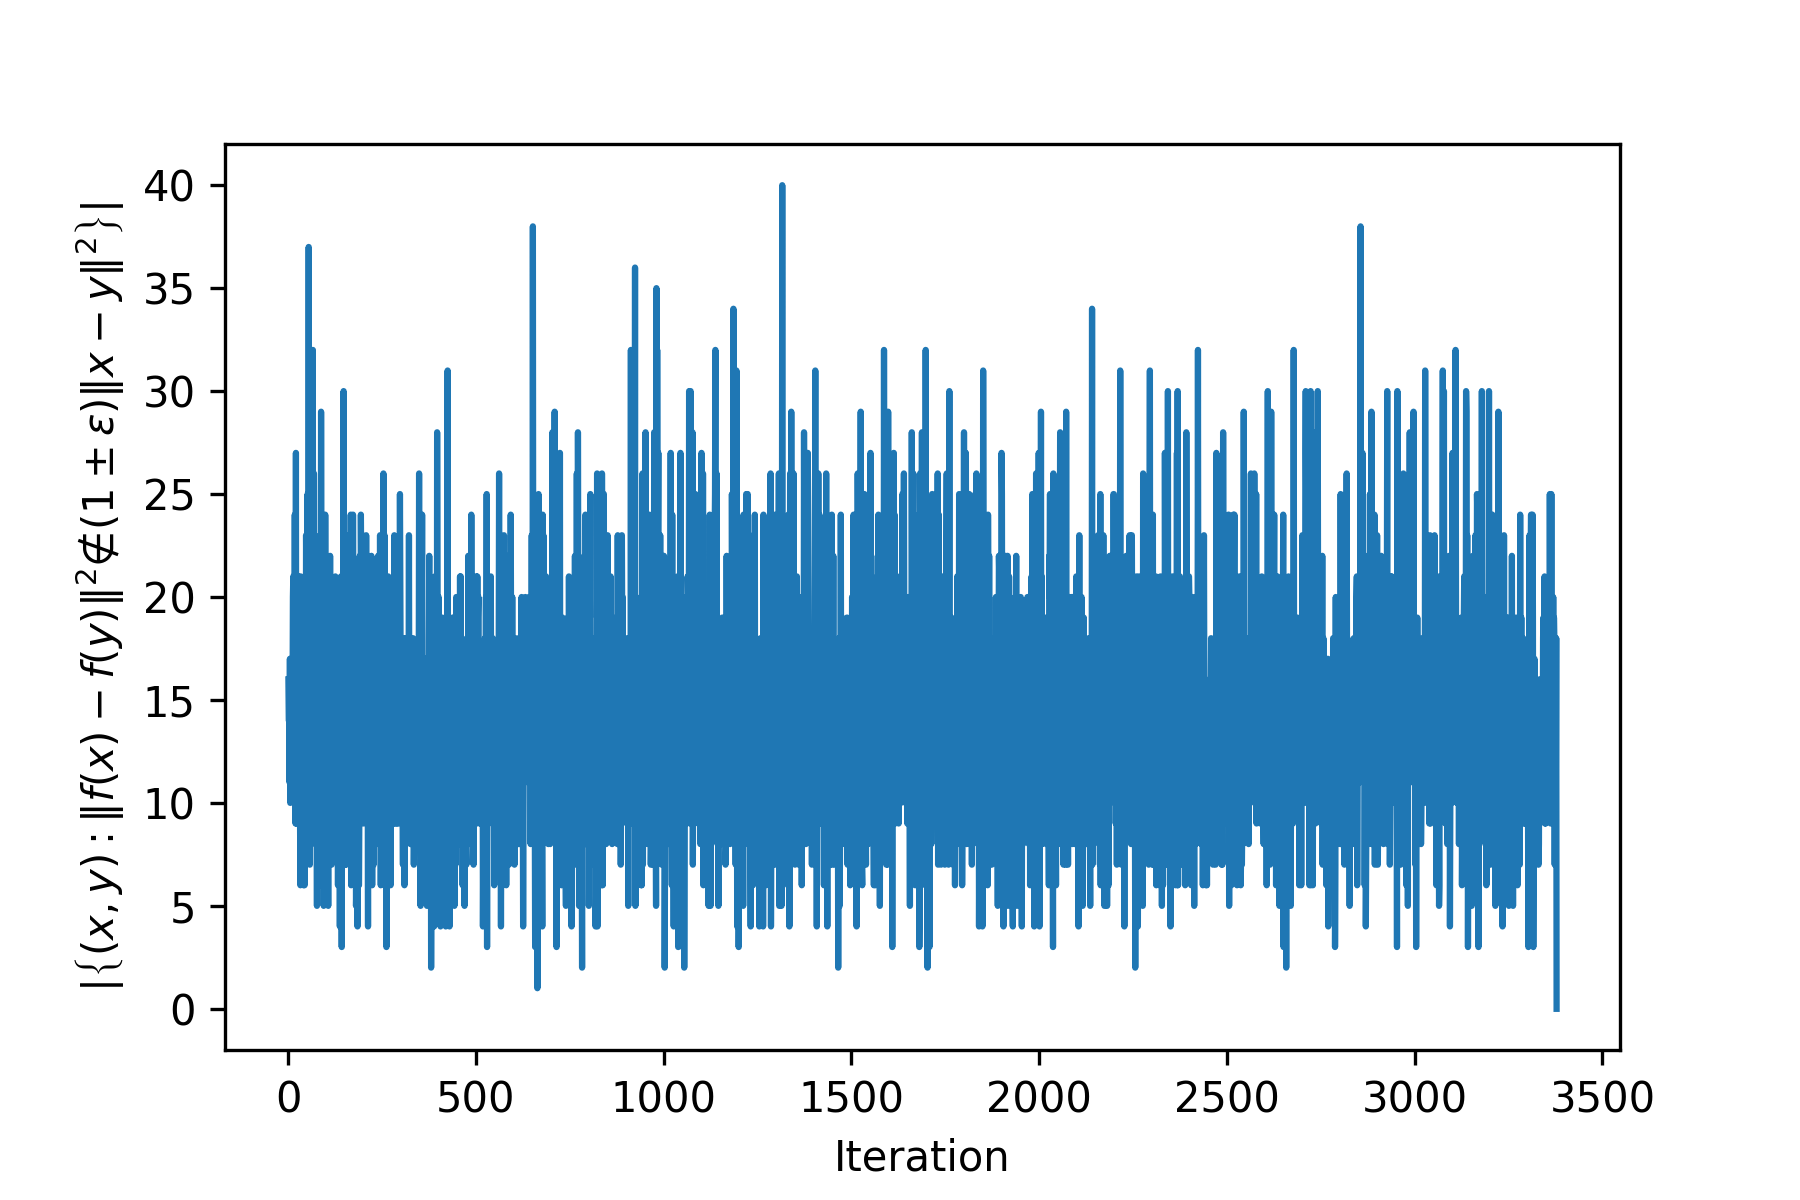
\includegraphics[width=.9\textwidth]{imgs/jl_iterations.png}
    \caption{Number of pairs of points which do \textit{not} meet the desired distance-distortion criterion, plotted against the iterations of the JL algorithm; note that there $\binom{n}{2} = 190$ total pairs of points in $V$}
\end{figure}

\begin{figure}[H]
    \centering
    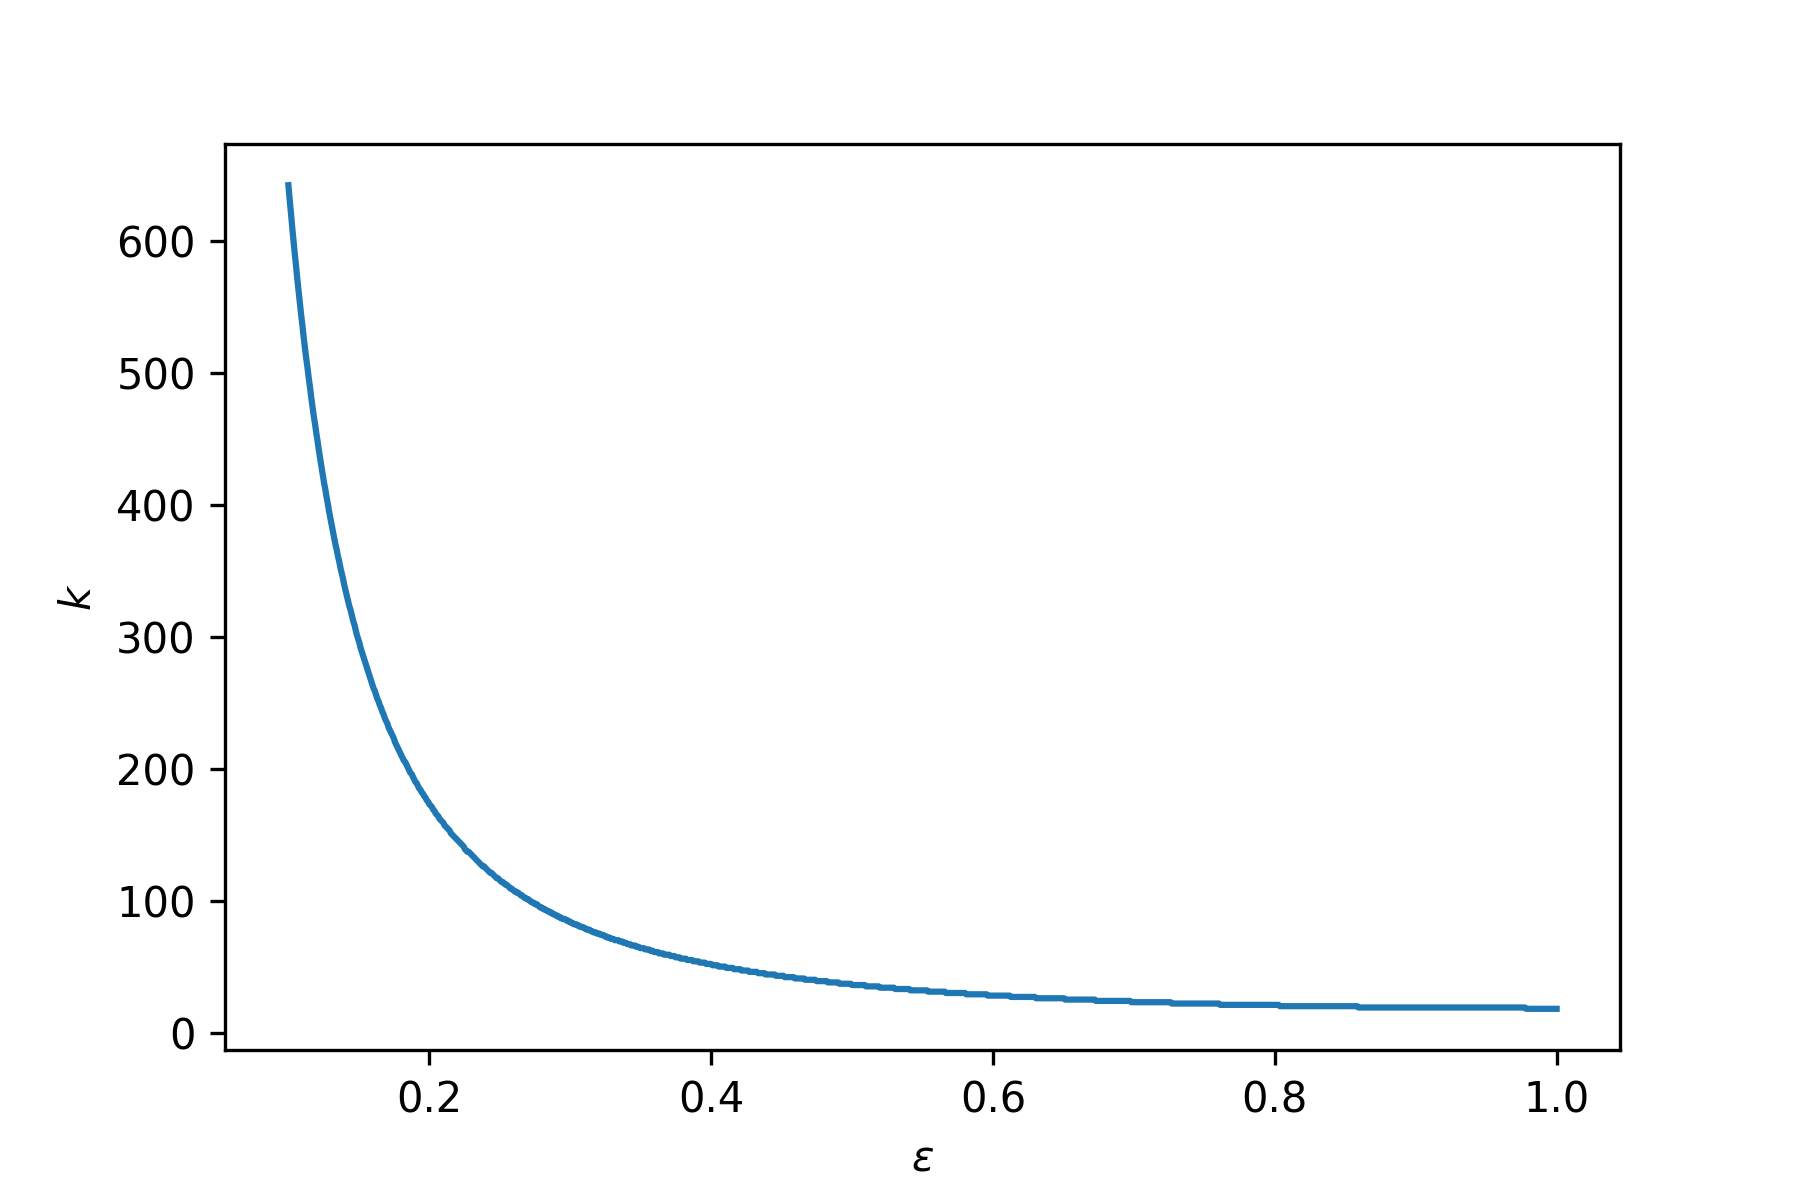
\includegraphics[width=.75\textwidth]{imgs/jl_dim_subspace.png}
    \caption{The minimum dimension $k$ such that the distance-preserving map $f: \mathbb{R}^d \rightarrow \mathbb{R}^k$ is gauranteed to exist by the Johnson-Lindenstrauss lemma versus the distance-distortion parameter $\epsilon$}
\end{figure}

\begin{figure}[H]
    \centering
    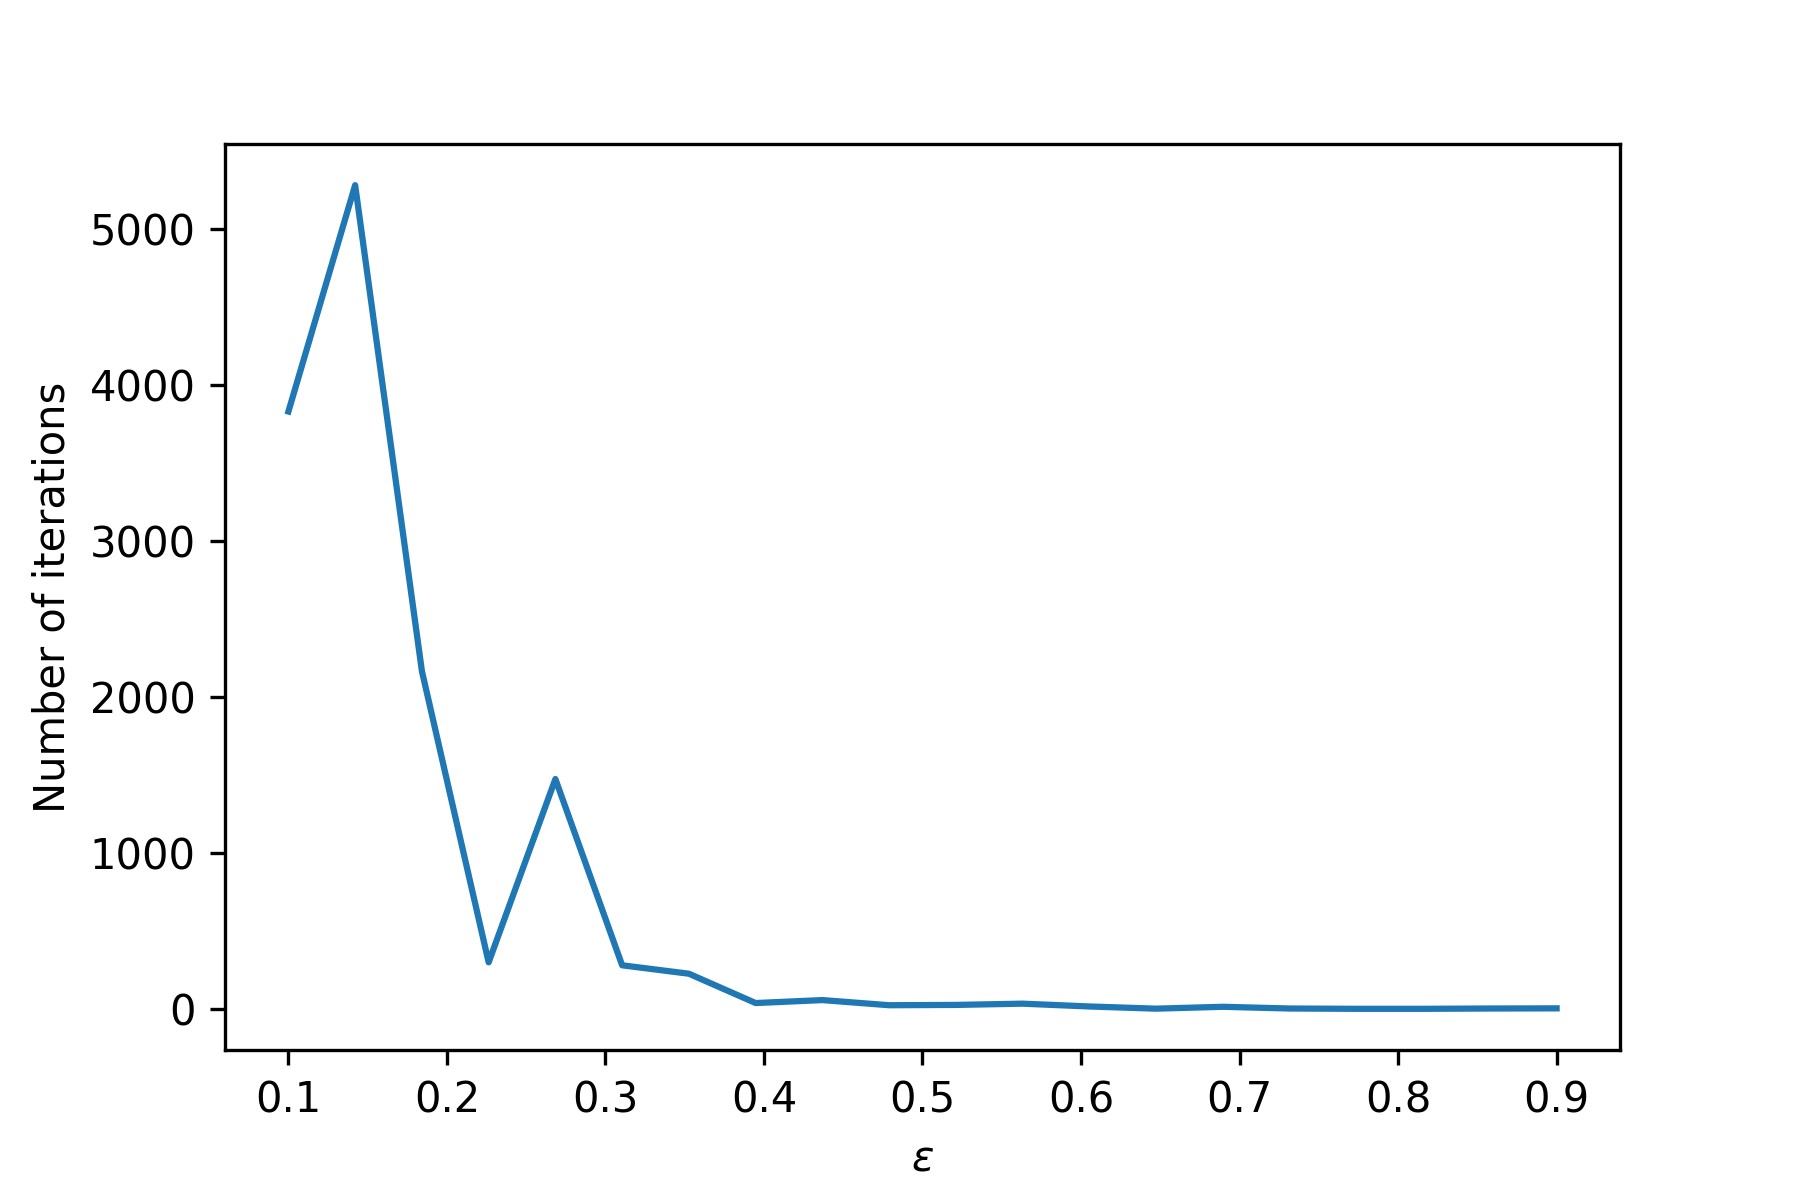
\includegraphics[width=.75\textwidth]{imgs/jl_num_iterations.png}
    \caption{Number of iterations to complete the JL algorithm versus distance distortion parameter $\epsilon$}
\end{figure}


\noindent
Perhaps unsurprisingly, our algorithm requires many iterations to find a random $k$-dimensional subspace that satisfies the distance-distortion property. Particularly, on one run, our algorithm considers $3348$ random $k$-dimensional subspaces of $\mathbb{R}^d$ before finding one which satisfies
$$(1 - \epsilon) \left \Vert x_i - x_j \right \Vert^2 \leq \left \Vert f(x_i) - f(x_j) \right \Vert^2 \leq (1 + \epsilon) \left \Vert x_i - x_j \right \Vert^2 \quad \forall x_i, x_j \in V.$$

\noindent
Notice from Figure 3 that the number of pairs of points that do not satisfy the above constraint at each iteration of the algorithm has no dependence on the how many iterations that algorithm has completed. This is what we would expect, since each iteration involves generating a new $k$-dimensional subspace of $\mathbb{R}^d$, independent of those previous subspaces. 

\noindent 
Further, in Figure 4 we see the relationship between $\epsilon$ and $k$ for this problem with $n = 20$ points. If one allows for greater distortion of the distances between points, then the dimension of the subspace onto which we may project decreases exponentially. 

\noindent
From Figure 5 we observe a clear relationship between the runtime of the algorithm and $\epsilon$. By increasing $\epsilon$, it is easier to find a random projection which satisfies the Johnson-Lindenstrauss distance distortion property. It is important to note, though, that there is no guaranteed runtime on the Johnson-Lindenstrauss algorithm. Since we are projecting our points in $\mathbb{R}^d$ onto \textit{randomized} $k$-dimensional subspaces, there exists the event that that we never find a subspace that meets the desired property. For this event, the Johnson-Lindenstrauss algorithm never terminates. Do be reassured, though, that this event has measure zero with respect to Lebesgue measure.


\newpage
\section{Johnson-Lindenstrauss vs Principal Components Analysis}

Although most people are are familiar with dimension reduction through Principal Components Analysis (PCA), random projections are another useful tool to reduce the dimension of a dataset. As a reminder, Principal Components Analysis involves projecting the centered data matrix
\begin{align*}
\widetilde{\mathbb{X}} = 
        \left[
            \begin{array}{ccc}
            \horzbar & \boldsymbol{x}_1 - \boldsymbol{\bar{x}} & \horzbar \\
            \horzbar & \boldsymbol{x}_2 - \boldsymbol{\bar{x}} & \horzbar \\
            & \vdots &  \\
            \horzbar & \boldsymbol{x}_n - \boldsymbol{\bar{x}} & \horzbar
            \end{array}
        \right] \qquad \text{where} \ \boldsymbol{\bar{x}}_i = \sum_{j=1}^n (\boldsymbol{x}_j)_i
\end{align*}
onto a $k$-dimensional subspace. In particular, each $\boldsymbol{x}_i - \boldsymbol{\bar{x}}$ is orthogonally projected onto the subspace spanned by $k$ eigenvectors of $\frac{1}{n}\widetilde{\mathbb{X}}^T\widetilde{\mathbb{X}}$. These $k$ eigenvectors are chosen to correspond to the $k$ largest eigenvalues of the matrix. This orthogonal projection onto the union of $k$ eigenspaces of $\frac{1}{n}\widetilde{\mathbb{X}}^T\widetilde{\mathbb{X}}$ preserves $(\sum_{i=1}^k \lambda_i/\sum_{i=1}^n \lambda_i \times 100)$\% of the original variance in the centered data.   

In general PCA remains the best option, but dimensionality reduction through the Johnson–Lindenstrauss algorithm may have some legitimate use cases as well.

For example, say we have a situation where we wish only to find the pairwise Euclidean distance between a large set of points with an extremely high dimensionality. This may be useful in situations such as the t-SNE embedding, a statistical method for visualizing high-dimensional data into two or three dimensions. In these situations, calculating pairwise distances with PCA would be prohibitively expensive due to the high-dimensionality of the data. This is not the case with random projections, as the Johnson–Lindenstrauss lemma guarantees the Euclidean distance within some error range \cite{stackoverflowpca}.

Specifically, we can consider the situation where we have a matrix of size $n \times d$. When projecting randomly, it requires $\mathcal{O}(ndk)$ operations to project on a subspace of dimension $k$. On the other hand, PCA takes $\mathcal{O}(d^2 \times n+d^3)$ operations \cite{stackoverflowpca}.

Additional cases where random projection may be preferable include when the data matrix under consideration is extremely sparse, or when memory is an issue (because you do not need to hold the data in memory for random projections, as opposed to PCA).

Overall, your use of dimensional reduction algorithm should depend on your specific needs. With a good understanding of the Johnson-Lindenstrauss lemma, we can add one more algorithm to our statistical toolkit.

\section{Appendix}
    \subsection{Generating Numbers from a Standard Normal Distribution}\label{stdnorm}
    Assume that we have an independent and random binary process. As discussed in class, this allows us to sample from the $\text{Uniform}(0,1)$ distribution. For each $k \in \mathbb{N}$, define $f(k)=0$ with probability $\frac{1}{2}$ and $1$ with probability $\frac{1}{2}$ which represents our binary process. Then, $x = \sum_{k=1}^\infty \frac{f(k)}{2^k}$ is a uniformly generated number in $[0,1]$. Given this existence of the uniform distribution, we show it is possible to randomly generate a value drawn from the $\mathcal{N}(0,1)$ distribution. Say that $X \sim \mathcal{N}(0,1)$. Let us investigate the distribution of $Y=F_X(X).$ Clearly the support of $Y$ is $[0,1]$ since $F_X(\cdot)$ outputs a probability. Furthermore, $F_X(x)$ is strictly monotonically increasing so it has an inverse. Using these facts,
    \begin{align*}
        F_Y(y) &= P(Y \leq y) \\
        &=P(F_X(X) \leq y)\\
        &=P(X \leq F_X^{-1}(y))\\
        &=F_X(F_X^{-1}(y))=y.
    \end{align*}
    This matches the CDF of the $\text{Uniform}(0,1)$ distribution: $Y \sim \text{Uniform}(0,1)$. Thus, if we wanted to go the other direction, it necessarily follows that $X = F_X^{-1}(Y)$ has a $\mathcal{N}(0,1)$ distribution where $F_X(x) = \int_{-\infty}^x \frac{1}{\sqrt{2\pi}}e^{-\frac{t^2}{2}}dt.$ This process can be used to generate each $A_{ij}$ which in turn will generate all of $\mathbb{A}$ as desired.
    
    \subsection{The Moment-Generating Function (MGF) of $\chi^2_n$}
Our results are made easier by finding the MGF of the $\chi_n^2$ distribution for any finite $n$. We will derive the result here. Notice by definition that if $Z \sim \chi^2_n$, then $Z = \sum_{i=1}^n Z_i^2$ where each $Z_i \overset{iid}{\sim} \mathcal{N}(0,1)$. Then 
\begin{align*}
    \mathbb{E}[e^{tZ}]&=\mathbb{E}[e^{t\sum_{i=1}^n Z_i^2}]\\
    &=\mathbb{E}[e^{tZ_1^2}e^{tZ_2^2}\ldots e^{tZ_n^2}]\\
    &=\mathbb{E}[e^{tZ_1^2}]\mathbb{E}[e^{tZ_n^2}]\ldots\mathbb{E}[e^{tZ_n^2}] & \text{the $Z_i$ are independent}\\
    &=(\mathbb{E}[e^{tZ_1^2}])^n. & \text{the $Z_i$ are identically distributed}
\end{align*}
Thus, we really only need to find $\mathbb{E}[e^{tZ_1^2}]$. This can be written as $\int_{-\infty}^\infty \frac{1}{\sqrt{2\pi}} e^{-\frac{x^2}{2}+tx^2}dx.$ 
\begin{align*}
  \int_{-\infty}^\infty \frac{1}{\sqrt{2\pi}} e^{-\frac{x^2}{2}+tx^2}dx&=
  \int_{-\infty}^\infty \frac{1}{\sqrt{2\pi}} e^{-\frac{x^2}{2\cdot (1/(1-2t))}}\\
  &=\int_{-\infty}^\infty \frac{\sqrt{1-2t}}{\sqrt{2\pi(1-2t)}} e^{-\frac{x^2}{2\cdot (1/(1-2t))}}\\
  &=\frac{1}{\sqrt{1-2t}}
\end{align*}
where the last equality comes the fact that the integral of the pdf of the $\mathcal{N}(0,\frac{1}{1-2t})$ distribution is $1$. Thus, the MGF of $Z \sim \chi^2_n$ distribution is \begin{align*}
    (1-2t)^{-n/2} \quad \text{for $t<\frac{1}{2}$}.
\end{align*}
    \subsection{Bounding the Taylor Series of $\log(1+x)$}
The Taylor series for $\log(1+x)$ is $\log(1+x) = \sum_{n=1}^\infty \frac{(-1)^{n-1}x^n}{n}$ for $x \in (-1, 1]$. Our goal is to show that $\log(1+x)\leq \sum_{n=1}^N \frac{(-1)^{n-1}x^n}{n}$ where $N$ is an odd integer. Call $S_N = \sum_{n=1}^N \frac{(-1)^{n-1}x^n}{n}$ and $R_N = \log(1+x)-S_N$. Let $k$ be an index over the positive integers. Let us look at $\{s_{2k+1}\}$. It is monotonically decreasing: 
$$s_{2k+1}-s_{2k-1} = \frac{x^{2k+1}}{2k+1}-\frac{x^{2k}}{2k}=x^{2k}\cdot \frac{2kx-2k-1}{2k(2k+1)}.$$The above expression is negative when $x\leq 1+\frac{1}{2k}.$ Since we are only concerned with $x \in (-1,1],$ our sequence is monotonically decreasing. Similar steps show that $\{s_{2k}\}$ is a monotonic increasing sequence. However, notice that $\lim_{k \to \infty} (s_{2k+1}-s_{2k}) = \lim_{k \to \infty} \frac{x^{2k+1}}{2k+1}=0$ since the series converges. Thus, $\lim_{k \to \infty} s_{2k+1} = \lim_{k \to \infty} s_{2k}$ (limits exist since each is monotonic). This means that $\lim_{k \to \infty} s_{2k+1}=\log(1+x).$ However, since we proved that $\{s_{2k+1}\}$ is monotonic decreasing, we know that $\log(1+x) \leq \sum_{n=1}^N \frac{(-1)^{n-1}x^n}{n}$ where $N$ is an odd integer. Specifically, this tells us that $\log(1+x)\leq x-\frac{x^2}{2}+\frac{x^3}{3}$ for $x \in (-1,1]$. 

\newpage
\bibliographystyle{siam}
\bibliography{biblio}

\end{document}
